
\section{Results}


\subsection{Effect of spatial structure in PD and HD games}

In our first simulation experiment, we compared the effect of spatial structure on the persistence of cooperators in the PD and HD games. For the \textbf{PD game} we were able to reproduce the theoretical prediction that spatial structure enables cooperators to persist, even if cooperation is not an evolutionarily stable strategy in well-mixed populations. Our simulated spatial PD population with neighborhood size $= 8$ could maintain an average of $66.5\%$ cooperators ($\pm 1.12 \%$) at a cost-benefit ratio of $r = 0.05$. For higher cost-benefit ratios, however, cooperation was not evolutionarily stable at this neighborhood size and ceased within the 5000 time steps. If cooperation did was cost-free, the proportion of cooperators remained close to its initial value. See figure \ref{fig: task1_4plot} for a comparison of the frequency of cooperation in spatial and nonspatial PD games.\\
In the spatial \textbf{HD game} we found a quite contrary effect of spatial structure. When simulating a well-mixed population we could reproduce the theoretical prediction that the equilibrium frequency of cooperators is $f(wm)=1 - r$. However, adding spatial structure to the model reduced the frequency of cooperators as compared to the non-spatial version for most r values (figure \ref{fig: task1_4plot}). 
\begin{figure}[H]
	\centering 
	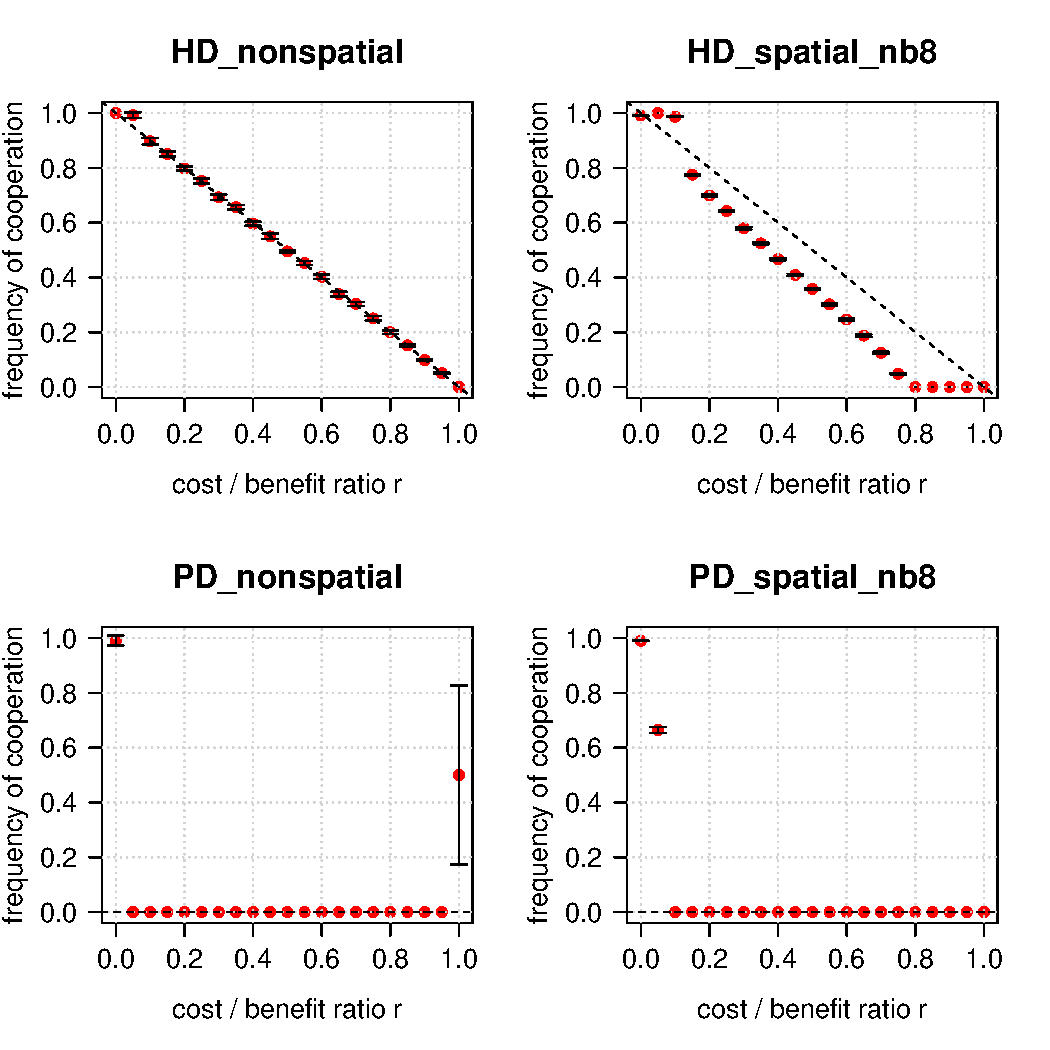
\includegraphics[width=9.5cm]{task1_4plot}
	\caption{Comparison of HD and PD game simulations, both with and without spatial structure. [ t = 5000, i = 10, error bars with 95\% confidence]} }\label{fig: task1_4plot}
\end{figure}
The higher the r value, the bigger the relative disadvantage of cooperators was. For $r \geq 0.8$ cooperation completely vanished from the population. Only at very low cost-benefit ratios, cooperators in the HD game profited from spatial structure. The threshold r value up to which cooperators profited was 0.1 for a neighborhood size of 8.



\subsection{Effect of neighborhood size}

In the second simulation experiment we varied neighborhood size in the spatial PD and HD games and investigated whether changes in neighborhood size would change the effects of spatiality. Except for neighborhood size, the HD simulations were run with the exact same parameter set as before. In the first PD game simulation spatial structure only came into effect at very small r-values. To achieve a reasonably high x-axis resolution in the most relevant section, we lowered the r-stepwidth from $0.05$ to $0.01$ for r-values $< 0.1$ in the second PD experiment.
% Move last two sentences to figure caption?

\subsubsection*{Spatial Hawk-Dove games}
Varying neighborhood size in the HD game yielded three main observations:\\ 
In the spatial HD game with eight neighbors, cooperators profited from spatial structure at low cost-benefit ratios and suffered at higher r-values. This also goes for different neighborhood sizes. However, the threshold r-value at which benefit turns into disadvantage varies with neighborhood size: It is higher for small neighborhood sizes and decreases with increasing neighborhood size.\\
In addition to the increased benefit from spatial structure at small r-values, smaller neighborhood sizes ($4$ neighbors) had another effect in the second HD experiment: The detriment of spatial structure in comparison to well-mixed populations increased faster for r-values above the threshold r-value. In contrast, bigger neighborhoods ($>8$ neighbors) were less detrimental to cooperators at high r-values.\\
At the upper end of the range of r-values, another effect of neighborhood size became apparent: The r-value above which total extinction of cooperators becomes likely changed with neighborhood size. The smaller the neighborhood, the more likely cooperators are to die out completely. With $N$ being the average number of neighbors, cooperators were likely to die out completely if $1 / N > 1 - r$. The effects of varying neighborhood sizes in the HD game are illustrated in figure \ref{fig: task2_4plot}.\\


\begin{figure}[H]
	\centering 
	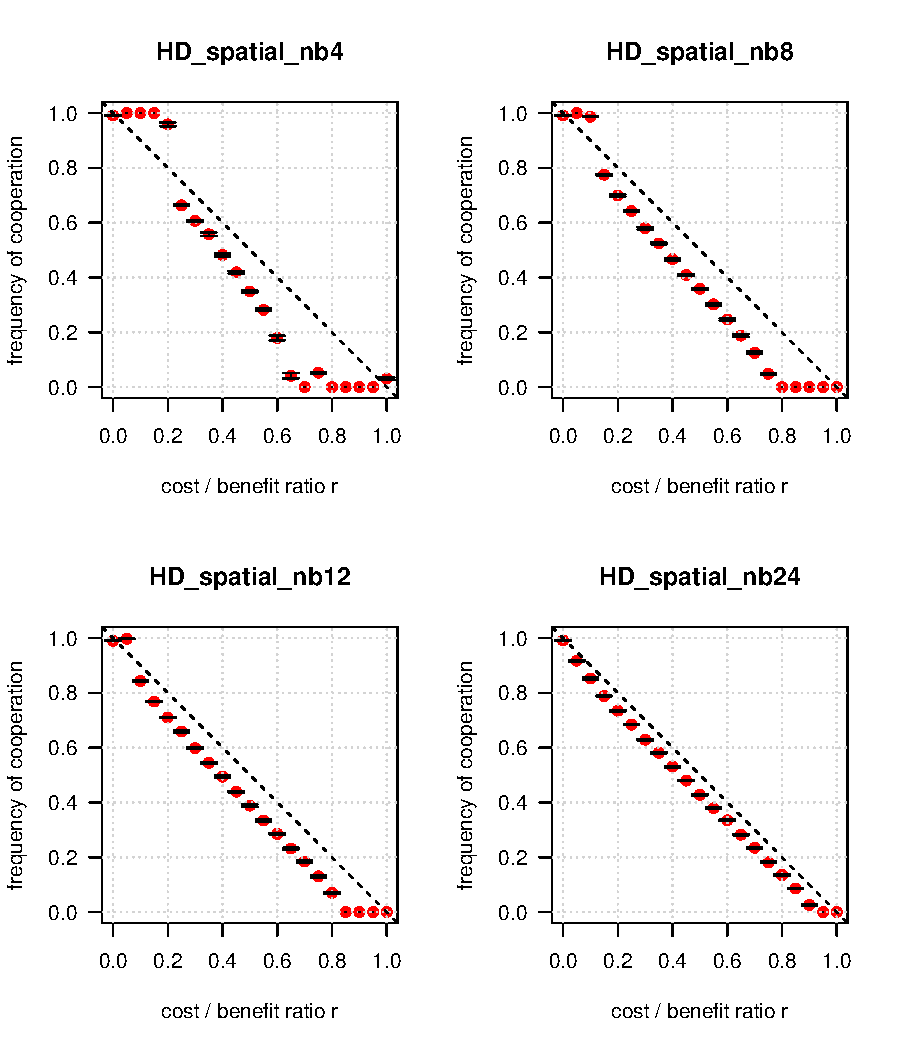
\includegraphics[width=9.5cm]{task2_4plot}
	\caption{Effect of varying neighborhood size in the HD game. The red dots represent the mean simulated values for the spatial HD game with 95\% confidence intervals. The dashed line represents cooperation frequency in a well-mixed population. [ t = 5000, i = 10 ] }\label{fig: task2_4plot}
\end{figure}



\subsubsection*{Spatial Prisoner's Dilemma games}
For all simulated neighborhood sizes, we could reproduce our finding from the first experiment: Spatial structure allows for the evolution of cooperation in PD games. Nonetheless, our second experiment revealed some constraints to this finding: Firstly, cooperation is only evolutionarily stable for r-values $ \leq 0.09$, for bigger r-values it disappears from the population. Secondly, neighborhood size has a big influence on a population's ability to maintain cooperation.\\
In very small neighborhoods ($4$ neighbors), cooperators are generally much less likely to persist and therefore make up for smaller ratios of the population than in bigger neighborhoods (see figure \ref{fig: task2_multiplot}). The extinction threshold for cooperators is at $r=0.04$ and thereby significantly lower than in bigger neighborhoods. 

\begin{figure}
	\centering 
	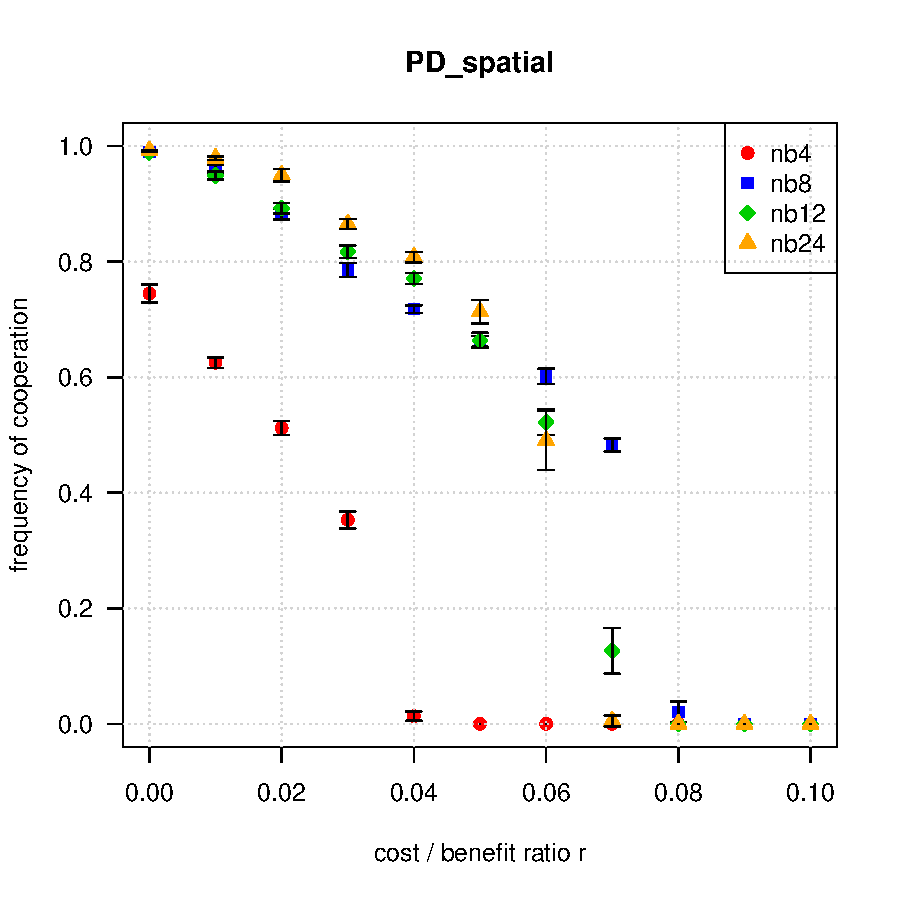
\includegraphics[width=9.5cm]{task2_multiplot}
	\caption{Spatial PD game simulations with different neighborhood sizes. The X-axis is cut off at $0.1$ as for all higher r-values, the frequency of cooperation was $0$. [ t = 5000, i = 10 ] }\label{fig: task2_multiplot}
\end{figure}
 
\noindent For neighborhood sizes of $8$ or more neighbors, however, the results are ambiguous: Up to a threshold of $r=0.05$, bigger neighborhoods result in slightly higher numbers of cooperators. At r-values between $0.05$ and $0.08$ however, the order inverts so that populations with neighborhood size $8$ can maintain more cooperation than those with neighborhood size $12$ or $24$. \\ 
Figure \ref{fig: task2_radiusplot} better illustrates this anomality: We ran the spatial PD game for two fixed r-values below ($0.03$) and above ($0.065$) the tipping point and at the same time varied neighborhood size. When looking at the results, it becomes apparent that at r-values close to the extinction threshold, the population with neighborhood size $=8$ constitutes an optimum for cooperators whereas populations with bigger neighborhood size can not maintain the high ratio of cooperators they supported at lower r-values.


\begin{figure}[H]
	\centering 
	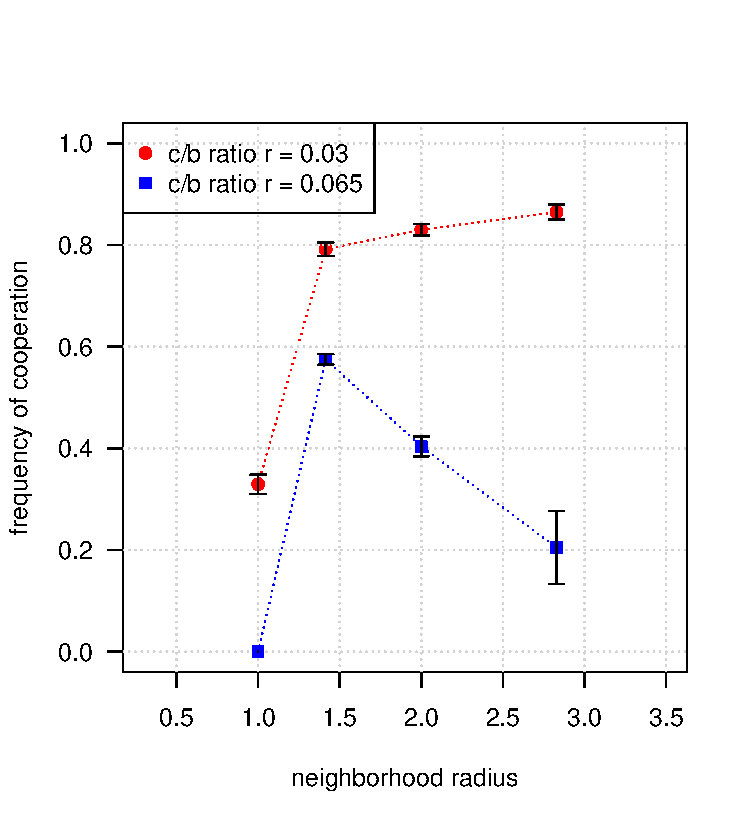
\includegraphics[width=9.5cm]{task2_radiusplot}
	\caption{Spatial PD game simulations with fixed cost-benefit-ratio and different neighborhood sizes. Radius 1 is adequate to 4 neighbors, radius 1.4 = 8 neighbors, radius 2 = 12 neighbors and radius 2.8 = 24 neighbors. [ t = 10000, i = 10 ] }\label{fig: task2_radiusplot}
\end{figure}




\subsection{Effect of mixed strategies in the Hawk-Dove game}
In our third experiment, we implemented mixed strategies in the HD game in order to compare the effect of spatial structure in the mixed-strategy HD game with that in the pure-strategy game. In the pure-strategy HD game, spatial structure lowers the ration of cooperators, except for very small r-values where it benefits them. In mixed-strategy HD games however, this ambivalence does not exist. For any r-values the probability to play cooperator is reduced in comparison to the non-spatial version of the game. However, the detriment of spatial structure on cooperators is not as severe as in the pure-strategy HD game, especially at high r-values (figure \ref*{fig: task3_multiplot}).\\ 
The general effect of varying neighborhood size is similar to the pure-strategy HD game: Bigger neighborhoods reduce the detriment of spatial structure to cooperators. As the frequency of cooperators in the mixed-strategy HD game is very close to their $1-r$ frequency in well-mixed populations anyway, the change induced by varying neighborhood size becomes negligibly small.



\begin{figure}[H]
	\centering 
	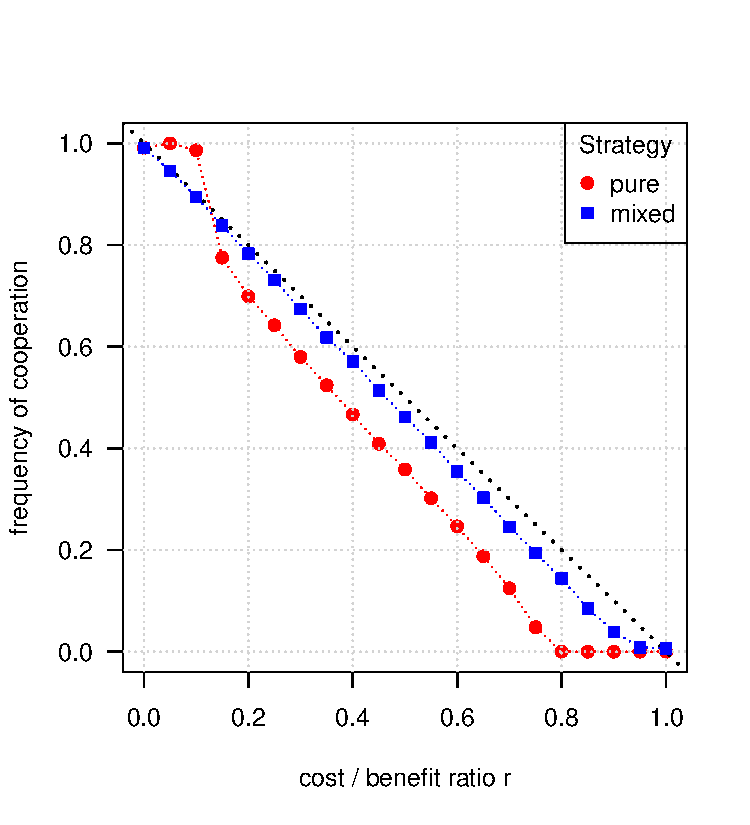
\includegraphics[width=9.5cm]{task3_multiplot}
	\caption{Spatial HD game simulations with neighborhood size = 8 and different strategies. The dotted black line depicts the frequency of cooperation in non-spatial HD games which equals $1-r$ for both pure- and mixed-strategy games. [ t = 10000, i = 10 ] }\label{fig: task3_multiplot}
\end{figure}






